\documentclass[t,usenames,dvipsnames]{beamer}
\usetheme{Copenhagen}
\setbeamertemplate{headline}{} % remove toc from headers
\beamertemplatenavigationsymbolsempty

\usepackage{amsmath, tkz-euclide, tikz, xcolor, pgfplots, array}
\usetkzobj{all}
\pgfplotsset{compat = 1.16}
\usetikzlibrary{arrows.meta, calc, decorations.pathreplacing}
\pgfplotsset{every axis/.append style = {axis lines = middle, axis line style = {<->}}}
\pgfplotsset{every tick label/.append style={font=\scriptsize}}
\everymath{\displaystyle}

\title{Inverse Trig Functions}
\author{}
\date{}

\AtBeginSection[]
{
  \begin{frame}
    \frametitle{Objectives}
    \tableofcontents[currentsection]
  \end{frame}
}

\begin{document}

\begin{frame}
    \maketitle
\end{frame}

\section{Find the values of inverse trig functions}

\begin{frame}{Trig Functions and the Horizontal Line Test}
Recall that for a function to have an \alert{inverse}, any horizontal line can only hit the function \underline{at most once}.  \newline\\  \pause

This creates a problem with periodic functions such as $y = \sin x$.
\end{frame}

\begin{frame}{Graph of $y=\sin x$ and $y = \frac{1}{2}$}
\begin{center}
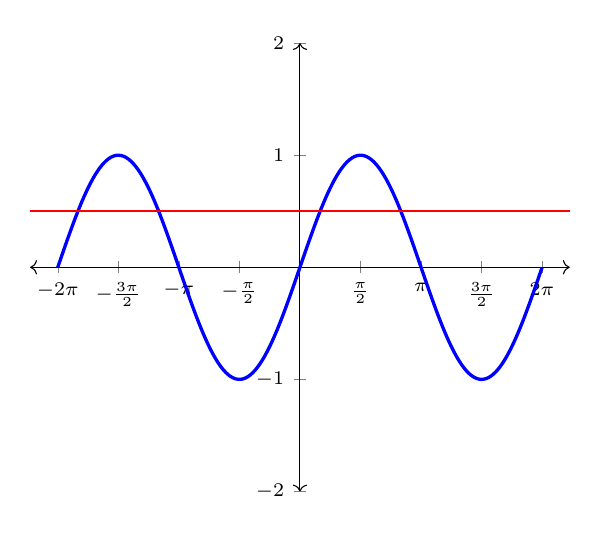
\begin{tikzpicture}
\begin{axis}[
    xmin = -7, xmax = 7,
    ymin = -2, ymax = 2,
    xtick = {-6.28, -4.71, -3.14, -1.57, 0, 1.57, 3.14, 4.71,  6.28},
    xticklabels = {$-2\pi$, $-\frac{3\pi}{2}$, $-\pi$, $-\frac{\pi}{2}$, , $\frac{\pi}{2}$, $\pi$, $\frac{3\pi}{2}$, $2\pi$}
]
\addplot [domain=-2*pi:2*pi, samples=200, smooth, very thick, color=blue] {sin(deg(x))};
\addplot [domain=-7:7, samples=200, smooth, thick, color=red] {0.5};
\end{axis}
\end{tikzpicture}
\end{center}
\end{frame}

\begin{frame}{Passing the Horizontal Line Test}
If we limit the graph to a smaller domain, then the Horizontal Line Test will demonstrate the function $y = \sin x$ will have an inverse: \newline\\  \pause

\begin{center}
\begin{tikzpicture}
\begin{axis}[
    xmin = -3.25, xmax = 3.25,
    ymin = -2, ymax = 2,
    xtick = {-3.14, -1.57, 0, 1.57, 3.14},
    xticklabels = {$-\pi$, $-\frac{\pi}{2}$, , $\frac{\pi}{2}$, $\pi$}
]
\addplot [domain=-pi/2:pi/2, samples=200, smooth, very thick, color=blue] {sin(deg(x))};
\end{axis}
\end{tikzpicture}
\end{center}
\end{frame}

\begin{frame}{Graph of $y = \sin^{-1} x$}
The inverse of $y=\sin x$ is 
\[
y = \sin^{-1}x \qquad \text{or} \qquad y = \arcsin x
\]  \pause
\begin{center}
\begin{tikzpicture}
\begin{axis}[
    xmin = -1.25, xmax = 1.25,
    ymin = -2, ymax = 2,
    domain = -1:1, samples=500,
    ytick = {-1.57,0,1.57},
    yticklabels = {$-\frac{\pi}{2}$,{}, $\frac{\pi}{2}$}
]
\addplot [very thick, color=blue] {asin(x)/180*pi};
\end{axis}
\end{tikzpicture}
\end{center}
\end{frame}

\begin{frame}{Domains and Ranges for Inverse Trig Functions}
\begin{center}
\setlength{\extrarowheight}{8pt}
\begin{tabular}{ccc}
\textbf{Inverse Function} & \textbf{Domain (Input)} & \textbf{Range (Output)} \\ \hline
\onslide<2->{$y = \sin^{-1} x$ & 
$[-1,1]$ & 
$\left[-\frac{\pi}{2},\frac{\pi}{2}\right]$} \\[10pt]
\onslide<3->{$y = \cos^{-1} x$ &
$[-1,1]$ &
$[0,\pi]$}   \\[10pt]
\onslide<4->{$y = \tan^{-1} x$ &
$(-\infty, \infty)$ &
$\left(-\frac{\pi}{2},\frac{\pi}{2}\right)$} \\[12pt]
\onslide<5->{$y = \csc^{-1} x$ &
$(-\infty, -1] \cup [1, \infty)$ &
$\left[-\frac{\pi}{2},0\right) \cup \left(0, \frac{\pi}{2}\right]$}  \\[10pt]
\onslide<6->{$y = \sec^{-1} x$ &
$(-\infty, -1] \cup [1, \infty)$ &
$\left[0, \frac{\pi}{2}\right) \cup \left(\frac{\pi}{2}, \pi\right]$} \\[12pt]
\onslide<7->{$y = \cot^{-1} x$ &
$(-\infty, \infty)$ &
$(0, \pi)$} \\
\end{tabular}
\end{center}
\end{frame}

\begin{frame}{Example 1}
Find the exact value of each.   \newline\\
(a) \quad $\sin^{-1}\left(\frac{\sqrt{2}}{2}\right)$    \newline\\
\begin{minipage}{0.5\textwidth} 
\vspace{18pt}
\onslide<2->{
\begin{tikzpicture}
\draw [<->] (-1,0) -- (3,0) node [right] {$x$};
\draw [<->] (0,-1) -- (0,2) node [above] {$y$};
\tkzDefPoints{0/0/A, 2/0/B, 2/1.5/C}
\tkzMarkRightAngle[color=red](C,B,A)
\tkzDrawPolygon(A,B,C)
\tkzLabelAngle[pos=0.5](B,A,C){\scriptsize $\theta$}
\tkzLabelSegment[right](B,C){\scriptsize $\sqrt{2}$}
\tkzLabelSegment(A,C){\scriptsize $2$}
\end{tikzpicture}}
\end{minipage}
\hspace{0.25cm}
\begin{minipage}{0.4\textwidth}
\begin{align*}
    \onslide<3->{\theta &= \sin^{-1}\left(\frac{\sqrt{2}}{2}\right)} \\[12pt]
    \onslide<4->{\theta &= 45^\circ} \\[12pt]
    \onslide<5->{\theta &= \frac{\pi}{4} }
\end{align*}
\end{minipage}
\end{frame}

\begin{frame}{Example 1}
Find the exact value of each.   \newline\\
(b) \quad $\cos^{-1}\left(-\frac{\sqrt{3}}{2}\right)$    \newline\\
\begin{minipage}{0.5\textwidth} 
\vspace{18pt}
\onslide<2->{
\begin{tikzpicture}
\draw [<->] (-3,0) -- (1,0) node [right] {$x$};
\draw [<->] (0,-1) -- (0,2) node [above] {$y$};
\tkzDefPoints{0/0/A, -2/0/B, -2/1.5/C}
\tkzMarkRightAngle[color=red](C,B,A)
\tkzDrawPolygon(A,B,C)
% \tkzLabelAngle[pos=0.5](B,A,C){\scriptsize $\theta$}
% \tkzLabelSegment[right](B,C){\scriptsize $\sqrt{2}$}
\tkzLabelSegment[below](A,B){\scriptsize $-\sqrt{3}$}
\tkzLabelSegment(A,C){\scriptsize $2$}
\draw [->] (0.5,0) arc (0:140:0.5) node [above right, xshift=0.5cm] {\scriptsize $\theta$};
\end{tikzpicture}}
\end{minipage}
\hspace{0.25cm}
\begin{minipage}{0.4\textwidth}
\begin{align*}
    \onslide<3->{\theta &= \cos^{-1}\left(\frac{-\sqrt{3}}{2}\right)} \\[12pt]
    \onslide<4->{\theta &= 150^\circ} \\[12pt]
    \onslide<5->{\theta &= \frac{5\pi}{6} }
\end{align*}
\end{minipage}
\end{frame}

\begin{frame}{Example 1}
Find the exact value of each.   \newline\\
(c) \quad $\arctan\left(\sqrt{3}\right)$    \newline\\
\begin{minipage}{0.5\textwidth} 
\vspace{18pt}
\onslide<2->{
\begin{tikzpicture}
\draw [<->] (-1,0) -- (3,0) node [right] {$x$};
\draw [<->] (0,-1) -- (0,2) node [above] {$y$};
\tkzDefPoints{0/0/A, 2/0/B, 2/1.5/C}
\tkzMarkRightAngle[color=red](C,B,A)
\tkzDrawPolygon(A,B,C)
\tkzLabelAngle[pos=0.5](B,A,C){\scriptsize $\theta$}
\tkzLabelSegment[right](B,C){\scriptsize $\sqrt{3}$}
\tkzLabelSegment[below](A,B){\scriptsize $1$}
\end{tikzpicture}}
\end{minipage}
\hspace{0.25cm}
\begin{minipage}{0.4\textwidth}
\begin{align*}
    \onslide<3->{\theta &= \arctan\left(\sqrt{3}\right)} \\[12pt]
    \onslide<4->{\theta &= 60^\circ} \\[12pt]
    \onslide<5->{\theta &= \frac{\pi}{3} }
\end{align*}
\end{minipage}
\end{frame}

\begin{frame}{Example 1}
Find the exact value of each.   \newline\\
(d) \quad $\sec^{-1}\left(2\right)$    \newline\\
\begin{minipage}{0.5\textwidth} 
\vspace{18pt}
\onslide<2->{
\begin{tikzpicture}
\draw [<->] (-1,0) -- (3,0) node [right] {$x$};
\draw [<->] (0,-1) -- (0,2) node [above] {$y$};
\tkzDefPoints{0/0/A, 2/0/B, 2/1.5/C}
\tkzMarkRightAngle[color=red](C,B,A)
\tkzDrawPolygon(A,B,C)
\tkzLabelAngle[pos=0.5](B,A,C){\scriptsize $\theta$}
\tkzLabelSegment[below](B,A){\scriptsize $1$}
\tkzLabelSegment[above](A,C){\scriptsize $2$}
\end{tikzpicture}}
\end{minipage}
\hspace{0.25cm}
\begin{minipage}{0.4\textwidth}
\begin{align*}
    \onslide<3->{\theta &= \sec^{-1}\left(2\right)} \\[12pt]
    \onslide<4->{\theta &= 60^\circ} \\[12pt]
    \onslide<5->{\theta &= \frac{\pi}{3} }
\end{align*}
\end{minipage}
\end{frame}


\section{Find the values of the compositions of inverse trig functions}


\begin{frame}{Compositions of Inverse Trig Functions}
When dealing with problems like these, it helps to \alert{sketch a right triangle}, much like in the previous example. \newline\\  

You may need to use the Pythagorean Theorem.
\end{frame}

\begin{frame}{Example 2}
Find the exact values of each (if possible).    \newline\\
(a) \quad $\cos\left(\cos^{-1}\left(\frac{1}{3}\right)\right)$  \newline\\
\begin{minipage}{0.5\textwidth} 
\vspace{18pt}
\onslide<2->{
\begin{tikzpicture}
\draw [<->] (-1,0) -- (3,0) node [right] {$x$};
\draw [<->] (0,-1) -- (0,2) node [above] {$y$};
\tkzDefPoints{0/0/A, 2/0/B, 2/1.5/C}
\tkzMarkRightAngle[color=red](C,B,A)
\tkzDrawPolygon(A,B,C)
\tkzLabelAngle[pos=0.5](B,A,C){\scriptsize $\theta$}
\tkzLabelSegment[below](B,A){\scriptsize $1$}
\tkzLabelSegment[above](A,C){\scriptsize $3$}
\end{tikzpicture}}
\end{minipage}
\hspace{0.25cm}
\begin{minipage}{0.4\textwidth}
\begin{align*}
    \onslide<3->{\theta &= \cos^{-1}\left(\frac{1}{3}\right)} \\[12pt]
    \onslide<4->{\cos\theta &= \frac{x}{r}} \\[12pt]
    \onslide<5->{\cos\theta &= \frac{1}{3} }
\end{align*}
\end{minipage}
\end{frame}


\begin{frame}{Example 2}
(b) \quad   $\sin\left(\arcsin\left(-\frac{3}{7}\right)\right)$   \newline\\    
\begin{minipage}{0.5\textwidth} 
\vspace{18pt}
\onslide<2->{
\begin{tikzpicture}
\draw [<->] (-1,0) -- (3,0) node [right] {$x$};
\draw [<->] (0,-2) -- (0,1) node [above] {$y$};
\tkzDefPoints{0/0/A, 2/0/B, 2/-1.5/C}
\tkzMarkRightAngle[color=red](C,B,A)
\tkzDrawPolygon(A,B,C)
\tkzLabelAngle[pos=0.5](B,A,C){\scriptsize $\theta$}
\tkzLabelSegment[right](B,C){\scriptsize $-3$}
\tkzLabelSegment[below](A,C){\scriptsize $7$}
\end{tikzpicture}}
\end{minipage}
\hspace{0.25cm}
\begin{minipage}{0.4\textwidth}
\begin{align*}
    \onslide<3->{\theta &= \arcsin\left(-\frac{3}{7}\right)} \\[12pt]
    \onslide<4->{\sin\theta &= \frac{y}{r}} \\[12pt]
    \onslide<5->{\sin\theta &= -\frac{3}{7} }
\end{align*}
\end{minipage}
\end{frame}


\begin{frame}{Example 2}
(c) \quad   $\cos\left(\arccos\left(\frac{5}{4}\right)\right)$   \newline\\    
\begin{minipage}{0.5\textwidth} 
\vspace{18pt}
\onslide<2->{
\begin{tikzpicture}
\draw [<->] (-1,0) -- (3,0) node [right] {$x$};
\draw [<->] (0,-1) -- (0,2) node [above] {$y$};
\tkzDefPoints{0/0/A, 2/0/B, 2/1.5/C}
\tkzMarkRightAngle[color=red](C,B,A)
\tkzDrawPolygon(A,B,C)
\tkzLabelAngle[pos=0.5](B,A,C){\scriptsize $\theta$}
\tkzLabelSegment[below](B,A){\scriptsize $5$}
\tkzLabelSegment[above](A,C){\scriptsize $4$}
\end{tikzpicture}}
\end{minipage}
\hspace{0.25cm}
\begin{minipage}{0.4\textwidth}
\begin{align*}
    \onslide<3->{\theta &= \arccos\left(\frac{5}{4}\right)} \\[12pt]
    \onslide<4->{&\text{Domain error.}} \\[12pt]
    \onslide<5->{&\varnothing}
\end{align*}
\end{minipage}
\end{frame}


\begin{frame}{Example 2}
(d) \quad   $\cos\left(\arctan\left(\frac{5}{12}\right)\right)$   \newline\\    
\begin{minipage}{0.5\textwidth} 
\vspace{18pt}
\onslide<2->{
\begin{tikzpicture}
\draw [<->] (-1,0) -- (3,0) node [right] {$x$};
\draw [<->] (0,-1) -- (0,2) node [above] {$y$};
\tkzDefPoints{0/0/A, 2/0/B, 2/1.5/C}
\tkzMarkRightAngle[color=red](C,B,A)
\tkzDrawPolygon(A,B,C)
\tkzLabelAngle[pos=0.5](B,A,C){\scriptsize $\theta$}
\tkzLabelSegment[below](B,A){\scriptsize $12$}
\tkzLabelSegment[right](B,C){\scriptsize $5$}
\onslide<5->{\tkzLabelSegment[above](A,C){\scriptsize $13$}}
\end{tikzpicture}}
\end{minipage}
\hspace{0.25cm}
\begin{minipage}{0.4\textwidth}
\begin{align*}
    \onslide<3->{\theta &= \arctan\left(\frac{5}{12}\right)} \\[12pt]
    \onslide<4->{12^2 + 5^2 &= r^2} \\[12pt]
    \onslide<5->{r &= \sqrt{169} = 13} \\[12pt]
    \onslide<6->{\cos\theta &= \frac{12}{13}}
\end{align*}
\end{minipage}
\end{frame}


\begin{frame}{Example 2}
(e) \quad   $\sin\left(\arctan\left(\frac{3}{4}\right)\right)$   \newline\\    
\begin{minipage}{0.5\textwidth} 
\vspace{18pt}
\onslide<2->{
\begin{tikzpicture}
\draw [<->] (-1,0) -- (3,0) node [right] {$x$};
\draw [<->] (0,-1) -- (0,2) node [above] {$y$};
\tkzDefPoints{0/0/A, 2/0/B, 2/1.5/C}
\tkzMarkRightAngle[color=red](C,B,A)
\tkzDrawPolygon(A,B,C)
\tkzLabelAngle[pos=0.5](B,A,C){\scriptsize $\theta$}
\tkzLabelSegment[below](B,A){\scriptsize $4$}
\tkzLabelSegment[right](B,C){\scriptsize $3$}
\onslide<5->{\tkzLabelSegment[above](A,C){\scriptsize $5$}}
\end{tikzpicture}}
\end{minipage}
\hspace{0.25cm}
\begin{minipage}{0.4\textwidth}
\begin{align*}
    \onslide<3->{\theta &= \arctan\left(\frac{3}{4}\right)} \\[12pt]
    \onslide<4->{3^2 + 4^2 &= r^2} \\[12pt]
    \onslide<5->{r &= \sqrt{25} = 5} \\[12pt]
    \onslide<6->{\sin\theta &= \frac{3}{5}}
\end{align*}
\end{minipage}
\end{frame}


\begin{frame}{Example 2}
(f) \quad   $\cot\left(\arcsin\left(-\frac{1}{3}\right)\right)$   \newline\\    
\begin{minipage}{0.5\textwidth} 
\vspace{18pt}
\onslide<2->{
\raisebox{1.5cm}{
\begin{tikzpicture}
\draw [<->] (-1,0) -- (3,0) node [right] {$x$};
\draw [<->] (0,-2) -- (0,1) node [above] {$y$};
\tkzDefPoints{0/0/A, 2/0/B, 2/-1.5/C}
\tkzMarkRightAngle[color=red](C,B,A)
\tkzDrawPolygon(A,B,C)
\tkzLabelAngle[pos=0.5](B,A,C){\scriptsize $\theta$}
\tkzLabelSegment[right](B,C){\scriptsize $-1$}
\tkzLabelSegment[below](A,C){\scriptsize $3$}
\onslide<5->{\tkzLabelSegment[above](B,A){\scriptsize $2\sqrt{2}$}}
\end{tikzpicture}} }
\end{minipage}
\hspace{0.25cm}
\begin{minipage}{0.4\textwidth}
\begin{align*}
    \onslide<3->{\theta &= \arcsin\left(-\frac{1}{3}\right)} \\[12pt]
    \onslide<4->{x^2 + 1^2 &= 3^2} \\[12pt]
    \onslide<5->{x &= \sqrt{8} = 2\sqrt{2}} \\[12pt]
    \onslide<6->{\cot\theta &= \frac{x}{y}} \\[12pt]
    \onslide<7->{\cot\theta &= \frac{2\sqrt{2}}{-1} = -2\sqrt{2}}
\end{align*}
\end{minipage}
\end{frame}

\begin{frame}{Example 2}
(g) \quad   $\sec\left(\arccos\left(\frac{3}{4}\right)\right)$   \newline\\    
\begin{minipage}{0.5\textwidth} 
\vspace{18pt}
\onslide<2->{
\begin{tikzpicture}
\draw [<->] (-1,0) -- (3,0) node [right] {$x$};
\draw [<->] (0,-1) -- (0,2) node [above] {$y$};
\tkzDefPoints{0/0/A, 2/0/B, 2/1.5/C}
\tkzMarkRightAngle[color=red](C,B,A)
\tkzDrawPolygon(A,B,C)
\tkzLabelAngle[pos=0.5](B,A,C){\scriptsize $\theta$}
\tkzLabelSegment[below](B,A){\scriptsize $3$}
\tkzLabelSegment[above](A,C){\scriptsize $4$}
\end{tikzpicture}}
\end{minipage}
\hspace{0.25cm}
\begin{minipage}{0.4\textwidth}
\begin{align*}
    \onslide<3->{\theta &= \arccos\left(\frac{3}{4}\right)} \\[12pt]
    \onslide<4->{\sec\theta &= \frac{r}{x}} \\[12pt]
    \onslide<5->{\sec\theta &= \frac{4}{3}}
\end{align*}
\end{minipage}
\end{frame}


\section{Write an algebraic expression for the compositions of inverse trig functions}

\begin{frame}{Algebraic Inverse Trig}
In calculus, inverse trigonometric functions will be expressed algebraically (i.e. in terms of $x$).    \newline\\

Set up a right triangle and use the \alert{Pythagorean Theorem} to write the missing side in terms of $x$.
\end{frame}

\begin{frame}{Example 3}
Write each as an algebraic expression of $x$.   \newline\\
(a) \quad   $\cos\left(\sin^{-1} x\right)$  \newline\\
\begin{minipage}{0.5\textwidth} 
\vspace{18pt}
\onslide<2->{
\raisebox{1.5cm}{
\begin{tikzpicture}
\draw [<->] (-1,0) -- (3,0) node [right] {$x$};
\draw [<->] (0,-1) -- (0,2) node [above] {$y$};
\tkzDefPoints{0/0/A, 2/0/B, 2/1.5/C}
\tkzMarkRightAngle[color=red](C,B,A)
\tkzDrawPolygon(A,B,C)
\tkzLabelAngle[pos=0.5](B,A,C){\scriptsize $\theta$}
\tkzLabelSegment[right](B,C){\scriptsize $x$}
\tkzLabelSegment[above](A,C){\scriptsize $1$}
\onslide<5->{\tkzLabelSegment[below](B,A){\scriptsize $\sqrt{1-x^2}$}}
\end{tikzpicture}} }
\end{minipage}
\hspace{-0.25cm}
\begin{minipage}{0.4\textwidth}
\begin{align*}
    \onslide<3->{\theta &= \arcsin\left(x\right)} \\[8pt]
    \onslide<4->{a^2 + x^2 &= 1^2} \\[8pt]
    \onslide<5->{a &= \sqrt{1-x^2}} \\[8pt]
    \onslide<6->{\cos\theta &= \frac{\text{adj}}{\text{hyp}}} \\[12pt]
    \onslide<7->{\cos\theta &= \frac{\sqrt{1-x^2}}{1} = -\sqrt{1-x^2}}
\end{align*}    
\end{minipage} 
\end{frame}

\begin{frame}{Example 3}
(b) \quad   $\sec\left(\tan^{-1} x\right)$  \newline\\
\begin{minipage}{0.5\textwidth} 
\vspace{18pt}
\onslide<2->{
\raisebox{1.5cm}{
\begin{tikzpicture}
\draw [<->] (-1,0) -- (3,0) node [right] {$x$};
\draw [<->] (0,-1) -- (0,2) node [above] {$y$};
\tkzDefPoints{0/0/A, 2/0/B, 2/1.5/C}
\tkzMarkRightAngle[color=red](C,B,A)
\tkzDrawPolygon(A,B,C)
\tkzLabelAngle[pos=0.5](B,A,C){\scriptsize $\theta$}
\tkzLabelSegment[right](B,C){\scriptsize $x$}
\onslide<5->{\tkzLabelSegment[above,sloped](A,C){\scriptsize $\sqrt{1+x^2}$}}
\tkzLabelSegment[below](B,A){\scriptsize $1$}
\end{tikzpicture}} }
\end{minipage}
\hspace{-0.25cm}
\begin{minipage}{0.4\textwidth}
\begin{align*}
    \onslide<3->{\theta &= \arctan\left(x\right)} \\[8pt]
    \onslide<4->{1^2 + x^2 &= c^2} \\[8pt]
    \onslide<5->{c &= \sqrt{1+x^2}} \\[8pt]
    \onslide<6->{\sec\theta &= \frac{\text{hyp}}{\text{adj}}} \\[12pt]
    \onslide<7->{\sec\theta &= \frac{\sqrt{1+x^2}}{1} = \sqrt{1+x^2}}
\end{align*}    
\end{minipage} 
\end{frame}

\begin{frame}{Example 3}
(c) \quad   $\tan\left(\sin^{-1}(2x)\right)$    \newline\\
\begin{minipage}{0.5\textwidth} 
\vspace{18pt}
\onslide<2->{
\raisebox{1.5cm}{
\begin{tikzpicture}
\draw [<->] (-1,0) -- (3,0) node [right] {$x$};
\draw [<->] (0,-1) -- (0,2) node [above] {$y$};
\tkzDefPoints{0/0/A, 2/0/B, 2/1.5/C}
\tkzMarkRightAngle[color=red](C,B,A)
\tkzDrawPolygon(A,B,C)
\tkzLabelAngle[pos=0.5](B,A,C){\scriptsize $\theta$}
\tkzLabelSegment[right](B,C){\scriptsize $2x$}
\tkzLabelSegment[above](A,C){\scriptsize $1$}
\onslide<6->{\tkzLabelSegment[below](B,A){\scriptsize $\sqrt{1-4x^2}$}}
\end{tikzpicture}} }
\end{minipage}
\hspace{-1cm}
\begin{minipage}{0.5\textwidth}
\begin{align*}
    \onslide<3->{\theta &= \arcsin\left(2x\right)} \\[12pt]
    \onslide<4->{a^2 + (2x)^2 &= 1^2} \\[12pt]
    \onslide<5->{a^2 + 4x^2 &= 1} \\[12pt]
    \onslide<6->{a &= \sqrt{1-4x^2}} 
\end{align*}
\end{minipage}
\end{frame}

\begin{frame}{Example 3}
(c) \quad   $\tan\left(\sin^{-1}(2x)\right)$    \newline\\
\begin{minipage}{0.5\textwidth} 
\vspace{18pt}
\raisebox{1.5cm}{
\begin{tikzpicture}
\draw [<->] (-1,0) -- (3,0) node [right] {$x$};
\draw [<->] (0,-1) -- (0,2) node [above] {$y$};
\tkzDefPoints{0/0/A, 2/0/B, 2/1.5/C}
\tkzMarkRightAngle[color=red](C,B,A)
\tkzDrawPolygon(A,B,C)
\tkzLabelAngle[pos=0.5](B,A,C){\scriptsize $\theta$}
\tkzLabelSegment[right](B,C){\scriptsize $2x$}
\tkzLabelSegment[above](A,C){\scriptsize $1$}
\tkzLabelSegment[below](B,A){\scriptsize $\sqrt{1-4x^2}$}
\end{tikzpicture}} 
\end{minipage}
\hspace{-1cm}
\begin{minipage}{0.5\textwidth}
\begin{align*}
    \onslide<2->{\tan\theta &= \frac{\text{opp}}{\text{adj}}} \\[15pt]
    \onslide<3->{\tan\theta &= \frac{2x}{\sqrt{1-4x^2}}}  \\[15pt]
    \onslide<4->{\tan\theta &= \frac{2x\sqrt{1-4x^2}}{1-4x^2}} 
\end{align*}    
\end{minipage} 
\end{frame}


\begin{frame}{Example 3}
(d) \quad $\sin\left(\cot^{-1}\left(\frac{x}{5}\right)\right)$  \newline\\
\begin{minipage}{0.5\textwidth} 
\vspace{18pt}
\onslide<2->{
\raisebox{1.5cm}{
\begin{tikzpicture}
\draw [<->] (-1,0) -- (3,0) node [right] {$x$};
\draw [<->] (0,-1) -- (0,2) node [above] {$y$};
\tkzDefPoints{0/0/A, 2/0/B, 2/1.5/C}
\tkzMarkRightAngle[color=red](C,B,A)
\tkzDrawPolygon(A,B,C)
\tkzLabelAngle[pos=0.5](B,A,C){\scriptsize $\theta$}
\tkzLabelSegment[right](B,C){\scriptsize $5$}
\onslide<5->{\tkzLabelSegment[above,sloped](A,C){\scriptsize $\sqrt{25+x^2}$}}
\tkzLabelSegment[below](B,A){\scriptsize $x$}
\end{tikzpicture}} }
\end{minipage}
\hspace{-0.25cm}
\begin{minipage}{0.4\textwidth}
\begin{align*}
    \onslide<3->{\theta &= \cot^{-1}\left(\frac{x}{5}\right)} \\[8pt]
    \onslide<4->{5^2 + x^2 &= c^2} \\[8pt]
    \onslide<5->{c &= \sqrt{25+x^2}}
\end{align*}    
\end{minipage} 
\end{frame}

\begin{frame}{Example 3}
(d) \quad $\sin\left(\cot^{-1}\left(\frac{x}{5}\right)\right)$  \newline\\
\begin{minipage}{0.5\textwidth} 
\vspace{18pt}
\raisebox{1.5cm}{
\begin{tikzpicture}
\draw [<->] (-1,0) -- (3,0) node [right] {$x$};
\draw [<->] (0,-1) -- (0,2) node [above] {$y$};
\tkzDefPoints{0/0/A, 2/0/B, 2/1.5/C}
\tkzMarkRightAngle[color=red](C,B,A)
\tkzDrawPolygon(A,B,C)
\tkzLabelAngle[pos=0.5](B,A,C){\scriptsize $\theta$}
\tkzLabelSegment[right](B,C){\scriptsize $5$}
\tkzLabelSegment[above,sloped](A,C){\scriptsize $\sqrt{25+x^2}$}
\tkzLabelSegment[below](B,A){\scriptsize $x$}
\end{tikzpicture}} 
\end{minipage}
\hspace{-0.25cm}
\begin{minipage}{0.4\textwidth}
\begin{align*}
    \onslide<2->{\sec\theta &= \frac{\text{hyp}}{\text{adj}}} \\[12pt]
    \onslide<3->{\sec\theta &= \frac{\sqrt{25+x^2}}{x}}
\end{align*}    
\end{minipage} 
\end{frame}


\end{document}
